\documentclass{article}
\usepackage[polish]{babel}
\usepackage{minted}
\usepackage[letterpaper,top=2cm,bottom=2cm,left=3cm,right=3cm,marginparwidth=1.75cm]{geometry}
\usepackage{amsmath}
\usepackage{graphicx}
\usepackage[colorlinks=true, allcolors=blue]{hyperref}
\usepackage[T1]{fontenc}
\usepackage[table,xcdraw]{xcolor}
\usepackage{float}
\usepackage[figurename=Wykres]{caption}
\usepackage{amsmath}
\graphicspath{{./images/}}

\title{MOwNiT - Rozwiązywanie układów równań liniowych metodami bezpośrednimi}

\author{Jakub Frączek}

\begin{document}

\maketitle

\section{Wstęp}

Tematem ćwiczenia było zaimplementowanie algorytmu Gaussa oraz Thomasa do rozwiązywania układów równań liniowych, a następnie rozwiązanie 3 ćwiczeń polegająćych na przeanalizowaniu wyników otrzymanych przy użyciu tych algorytmów w zależności od zadancyh układów oraz przyjętych precyzji oraz przygotowanie sprawozdania. 

\subsection{Ćwiczenie 1}

Dla macierzy zadanej wzorem:

\begin{equation}
  \begin{cases}
    a_{ij} = 1 , & \text{i != 1}.\\
    a_{ij} = 1 / (i + j - 1), & \text{otherwise}.
  \end{cases}
\end{equation}

\noindent
Gdzie \(i,j = 1,2,...n\)

\noindent
Przyjąć wektor X jako dowolną n-elementowąpermutacją ze zbioru {-1, 1} i obliczyć wektor B ze wzoru \(A \cdot X = B\). Następnie dla różnych precyzji i rozmiarów macierzy A i wektora B wyliczyć rozwiązanie ukłądu metodą Gaussa i porównać błędy zaokrągleń.

\subsection{Ćwiczenie 2}

\noindent
Dla macierzy danej wzorem:

\begin{equation*}
\left\{
\begin{array}{ll}
a_{ij} = \frac{2i}{j} & \text{dla } j \geq i \\
a_{ij} = a_{ji} & \text{dla } j < i
\end{array}
\right.
\qquad \text{dla } i, j = 1, \ldots, n
\end{equation*}

\noindent
Powtórzyć eksperyment z ćwiczenia 1, porównać różnice w wynikach i policzyć uwarunkowanie obu układów.

\subsection{Ćwiczenie 3}

\noindent
Dla macierzy danej wzorem:
\[
\left\{
\begin{array}{ll}
a_{i,j} = k \\
a_{i,j+1} = \frac{1}{i + m} & \\
a_{i+1,j} = \frac{k}{i + m + 1} & \text{dla } i > 1 \\
a_{i,j} = 0 & \text{dla } j < i - 1 \quad \text{oraz} \quad j > i + 1
\end{array}
\right.
\qquad i, j = 1, \ldots, n
\]

\noindent
Powtórzyć eksperyment z ćwiczenia 1 i 2, porównać różnice w wynikach oraz policzyć uwarunkowanie obu układów. Dodatkowo przeprowadzić analizę dla algorytmu \texttt{Thomasa} dla macierzy trójdiagonalnej.

\bigbreak

\noindent
Parametry \(k\) oraz \(m\) przydzielone w zadaniu indywidualnym wynosiły:

\[k = 6, \ m = 3\]

\newpage

\section{Dane techniczne}

\subsection{Hardware}

Do przeprowadzenia testów wykorzystany został laptop o następującej specyfikacji:

\begin{itemize}
    \item Procesor \texttt{Intel Core i5-9300H 2.4GHz}
    \item \texttt{32 GB} pamięci \texttt{RAM}.
\end{itemize}

\subsection{Software}

Wykorzystany został system \texttt{Windows 11 x64} oraz język \texttt{Python} w wersji \texttt{3.11.8} wraz z bibliotekami:
\begin{itemize}
\item \texttt{numpy}
\item \texttt{random}
\item \texttt{time}
\item \texttt{functools}
\item \texttt{typing}
\item \texttt{warning}
\end{itemize}

Do stworzenia wykresów wykorzystane zostało narzędzie \texttt{Google Sheets}.

\section{Wyznaczanie błędu obliczeń}

\noindent
Błąd obliczony został jako norma euklidesowa różnicy oczekiwanego i otrzymanego wektora.
Zakładając, że \(w_1\) to wynik wzorcowy, a \(w_2\) to wynik otrzymany za pomocą algorytmu \texttt{Gaussa} lub \texttt{Thomasa}m różnicę otrzymujemy w następujący sposób:

\[v = w_1 - w_1\]

\noindent
A następnie liczona jest z niej norma euklidesowa, którą przyjmuję jako błąd obliczeń.

\[\| \mathbf{v} \|_2 = \sqrt{v_1^2 + v_2^2 + \ldots + v_n^2}\]

\noindent
Funkcja wyliczająca normę z wektora została zaimplementowana przeze mnie.

\section{Wyznaczanie uwarunkowania układu}

Współczynnik uwarunkowania został obliczony według poniższego wzoru:

\[k(A) = ||A^{-1}|| \cdot |A|\]

\noindent
gdzie A - macierz zadana wzorem z ćwiczenia 1, 2 oraz 3

\bigbreak

\noindent
Ponownie funkcja wyliczająca normę z wektora została zaimplementowana przeze mnie, natomiast do wyznaczania odwrotności macierzy wykorzystałem funkcję \texttt{np.linalg.inv()} z biblioteki \texttt{numpy}.

\section{Sposób implementacji}

Algorytm Thomasa został zaimplementowany w wersji z oszczędnością pamięci. Tj. operuje na trzech listach zamiast na całej macierzy.

\bigbreak

\noindent
Implementacja obu algorytmów została zaadoptowana ze źródeł podanych w ostatnim paragrafie.

\section{Wyniki}

\noindent
Podczas przeprowadzania testów wykorzystałem dwie różne precyzje liczby zmiennoprzecinkowej udostępnione przez bibliotekę \texttt{numpy}:

\noindent
\begin{itemize}
    \item \texttt{np.float32}
    \item \texttt{np.float64}
\end{itemize}

\noindent
W miejscach, gdzie wykres w skali liniowej nie obrazował dobrze badanej zależności, wykorzystałem wykres w skali logarytminczej.

\subsection{Zadanie 1}

Jak widać na \texttt{wykresie 1} oraz \texttt{wykresie 2} błąd przybliżenia bardzo szybko rośnie wraz ze zwiększeniem rozmiaru układum dodatkowo błąd jest znacznie większy dla 64 bitowej precyzji. Generalnie przybliżenie jest złe.

\begin{figure}[H]
  \begin{minipage}[b]{0.49\textwidth}
    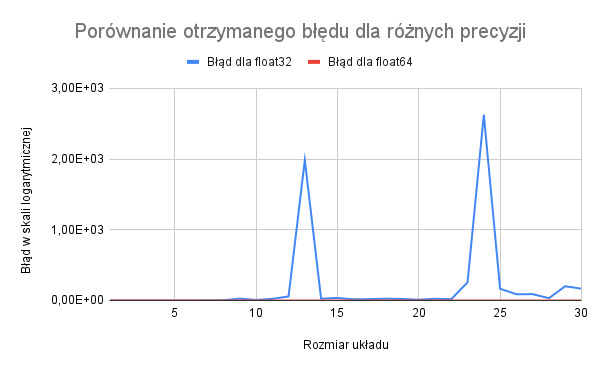
\includegraphics[width=\textwidth]{img01.png}
    \caption{Wykres błędu w zależności od przyjętej precyzji}
  \end{minipage}
  \hfill
  \begin{minipage}[b]{0.49\textwidth}
    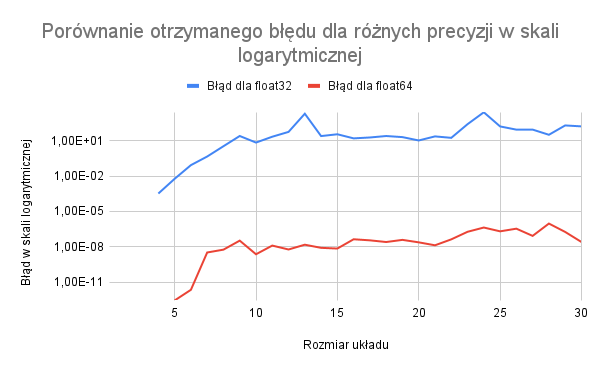
\includegraphics[width=\textwidth]{img02.png}
    \caption{Wykres błędu w zależności od przyjętej precyzji w skali logarytmicznej }
  \end{minipage}
\end{figure}

\noindent
Po przeanalizowaniu \texttt{Wykreu 3} okazało się, że  uwarunkowanie układu jest bardzo złe, a współczynnik uwarunkowania rośnie niezwykle szybko wraz z wzrostem rozmiaru układu. Na \texttt{wykresie 4} zaprezentowany jest czas działania algorymu. Jak można było się spodziewać algorytm działa w czasie sześciennym. Ciekawą rzeczą jest natomiast to, że algorytm wykonuje się nieznacznie szybciej dla wersji 64 bitowej. Dzieje się tak dlatego, że dla 32 bitowego float'a tracimy część informacji i wyznaczenie wyniku może zająć dłużej.

\begin{figure}[H]
  \begin{minipage}[b]{0.49\textwidth}
    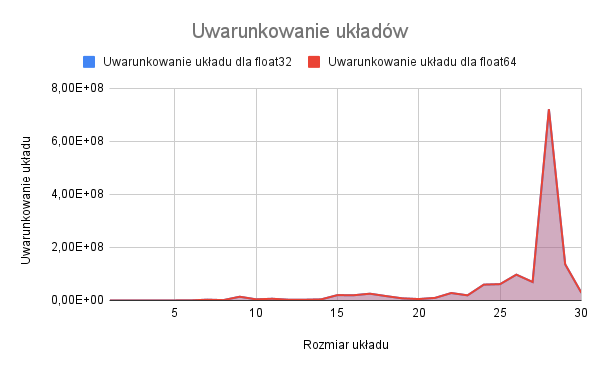
\includegraphics[width=\textwidth]{img03.png}
    \caption{Wykres uwarunkowania układu w skali logarytmicznej w zależności od przyjętej precyzji}
  \end{minipage}
  \hfill
  \begin{minipage}[b]{0.49\textwidth}
    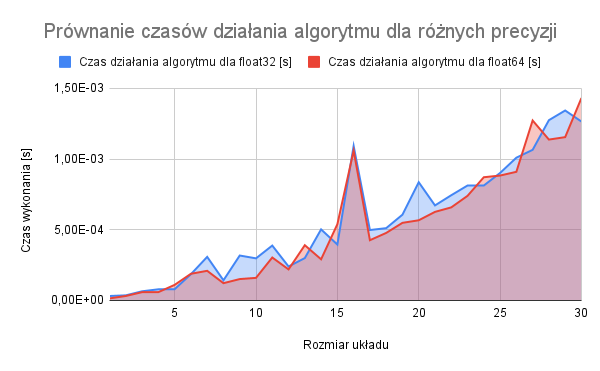
\includegraphics[width=\textwidth]{img04.png}
    \caption{Wykres czasów działania algorytmu w zależności od przyjętej precyzji}
  \end{minipage}
\end{figure}


\newpage

\subsection{Zadanie 2}

Jak widać na \texttt{Wykresie 5} i \texttt{Wykresie 6} błąd otrzymany dla 64 bitowej precyzji jest minimalny i rośnie bardzo powoli wraz z wzrostem rozmiaru układu. Błąd otrzymany dla 32 bitowej precyzji jest znacznie większy i rośńie dużo szybciej, jednak dla układu o rozmiarze 500 nadal jest on akceptowalny.

\begin{figure}[H]
  \begin{minipage}[b]{0.49\textwidth}
    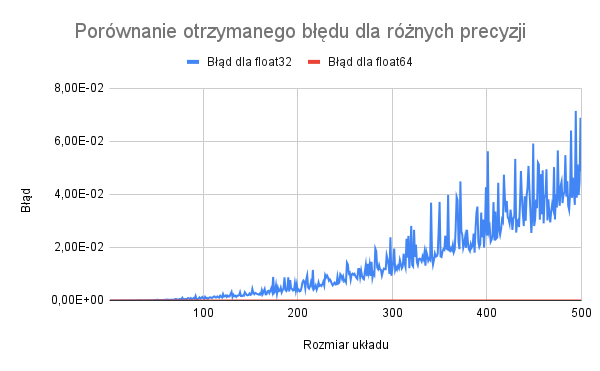
\includegraphics[width=\textwidth]{img05.png}
    \caption{Wykres błędu w zależności od przyjętej precyzji}
  \end{minipage}
  \hfill
  \begin{minipage}[b]{0.49\textwidth}
    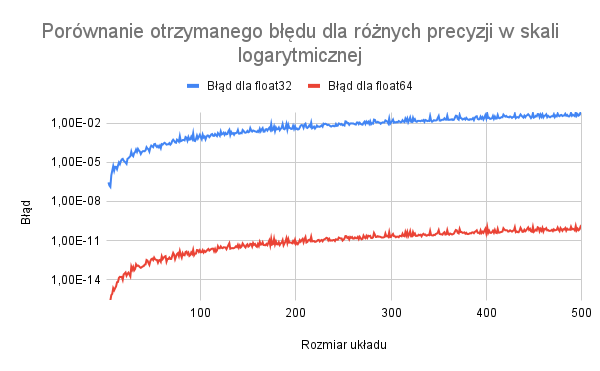
\includegraphics[width=\textwidth]{img06.png}
    \caption{Wykres błędu w zależności od przyjętej precyzji w skali logarytmicznej }
  \end{minipage}
\end{figure}

\noindent
Po spojrzeniu na \texttt{wykres 7} widać, że uwarunkowanie układu jest znacznie lepsze niż w przypadku zadania 1 i rośnie liniowo wraz z wzrostem rozmiaru układu. \texttt{Wykres 8} ponownie dowodzi sześciennej złożoności algorytmu, choć tym razem nie ma jasnej granicy pomiędzy czasami otrzymanymi dla różnych precyzji.

\begin{figure}[H]
  \begin{minipage}[b]{0.49\textwidth}
    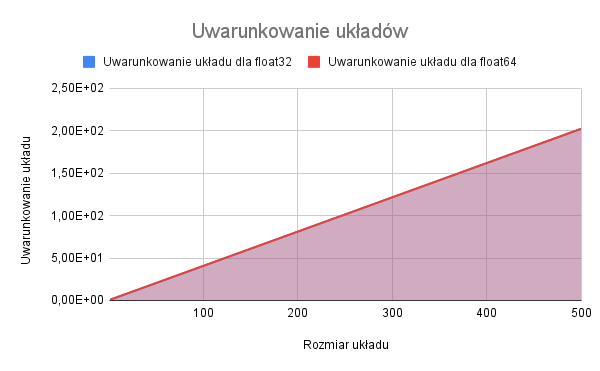
\includegraphics[width=\textwidth]{img07.png}
    \caption{Wykres uwarunkowania układu w skali logarytmicznej w zależności od przyjętej precyzji}
  \end{minipage}
  \hfill
  \begin{minipage}[b]{0.49\textwidth}
    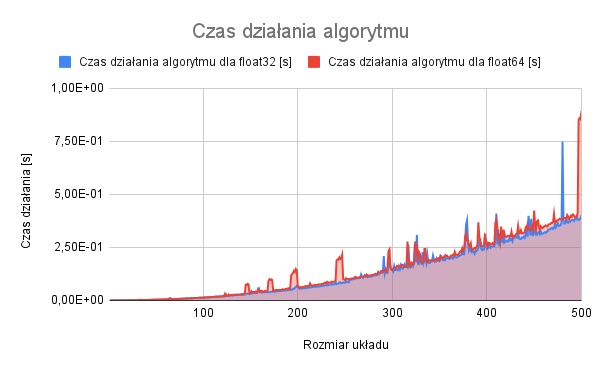
\includegraphics[width=\textwidth]{img08.png}
    \caption{Wykres czasów działania algorytmu w zależności od przyjętej precyzji}
  \end{minipage}
\end{figure}

\noindent
Na \texttt{wykresie 9} pokazane zostało porównanie pomiędzy uwarunkowaniem układu z zadania 1, a uwarunmkowaniem układu z zadania 2 dla rozmiarów układu od 1 do 30. Jak widać różnica jest kolosalna co potwierdza, że uwarunkowanie w zadaniu 2 jest znacznie lepsze.

\begin{figure}[H]
  \centering
    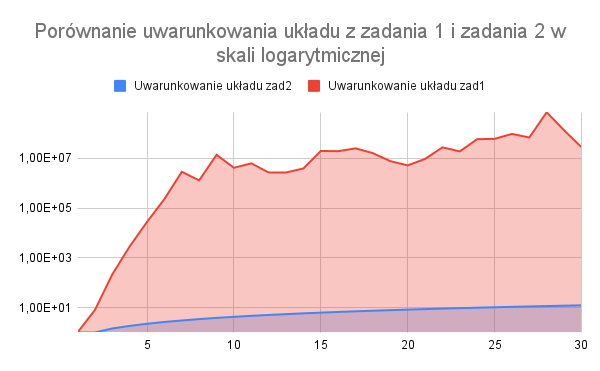
\includegraphics[width=0.4\textwidth]{img09.png}
  \caption{Porównanie uwarunkowania układu z zadania 1 i zadania 2 w skali logarytmicznej)}
\end{figure}

\newpage

\subsection{Zadanie 3a - float32}

\noindent
\texttt{Wykres 10} porównuje błąd otrzymany dla algrytmu \texttt{Thomasa} i algorytmu \texttt{Gaussa}. Jak widać, wartości błędów są bardzo zbliżone do siebie, jednak można zauważyć małą różnicę, która prawdopodobnie wynika ze sposobu implementacji obu algorytmów i różnicy w kolejności wykonanych operacji. Jak widać wraz ze wzrosem rozmiaru układu wartości nie odbiegają znacznie od siebie. Otrzymane błędy są bardzo małe i przybliżenie jest dobre.

\begin{figure}[H]
  \centering
    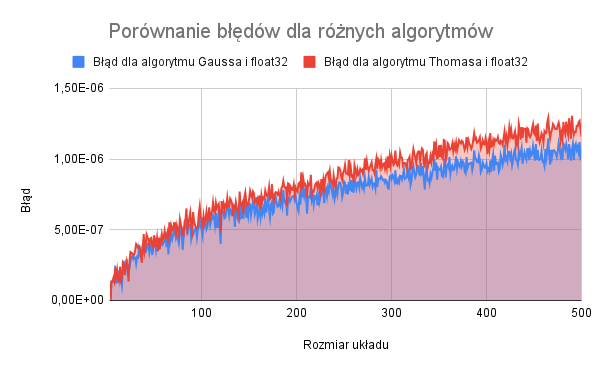
\includegraphics[width=0.8\textwidth]{img10.png}
  \caption{Wykres błędów dla algorytmu Gaussa i Thomasa oraz 32 bitowej precyzji}
\end{figure}

\texttt{Wykres 11} i \texttt{wykres 12} potwierdzają przewidywane złożoności tj. sześcienna dla algorytmu \texttt{Gaussa} i liniowa dla \texttt{Thomasa}. Dla dużych rozmiarów układu wykonanie algorytmu \texttt{Gaussa} zajmuje aż do 1 sekundy. 

\begin{figure}[H]
  \begin{minipage}[b]{0.49\textwidth}
    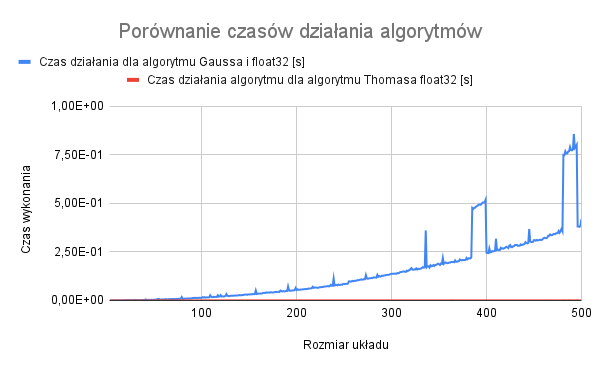
\includegraphics[width=\textwidth]{img11.png}
    \caption{Wykres czasów działania w zależności od przyjętej precyzji}
  \end{minipage}
  \hfill
  \begin{minipage}[b]{0.49\textwidth}
    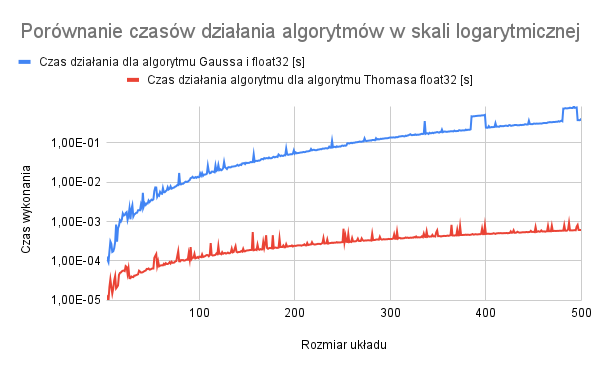
\includegraphics[width=\textwidth]{img12.png}
    \caption{Wykres czasów działania w skali logarytmicznej w zależności od przyjętej precyzji}
  \end{minipage}
\end{figure}

\noindent
Uuwarunkowanie układu jest bardzo dobre i nie zależy od jego rozmiaru.

\noindent
Wspołczynnik uwarunkowania dla zadania 3 wynosi:

\[k(A) = 1.16\]

\newpage

\subsection{Zadanie 3a - float64}

\noindent
\texttt{Wykres 13} porównuje błąd otrzymany dla algrytmu \texttt{Thomasa} i algorytmu \texttt{Gaussa}. Jak widać, wartości błędów są trochę mniej zbliżone do siebie niż w przypadku precyzji 32 bitowej (wykres 10). Ponownie różnica prawdopodobnie wynika ze sposobu implementacji obu algorytmów i różnicy w kolejności wykonanych operacji. Wraz ze wzrostem rozmiaru układu wartość błędów dla algorytmu Thomasa zwiększa się nieznacznie, jednak nadal jest ona bardzo mała, a otrzymany wynik jak najbardziej akceptowalny.

\begin{figure}[H]
  \centering
    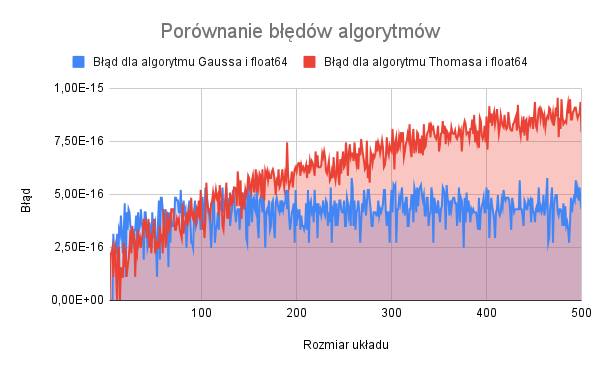
\includegraphics[width=0.8\textwidth]{images/img13.png}
  \caption{Wykres błędów dla algorytmu Gaussa i Thomasa oraz 64 bitowej precyzji}
\end{figure}

Ponownie \texttt{Wykres 14} i \texttt{wykres 15} potwierdzają przewidywane złożoności obliczeniowe algorytmu \texttt{Gaussa} i \texttt{Thomasa}. Wykonanie algorytmu Thomasa nawet dla bardzo dużych rozmiarów układu zajmuje ułamek sekundy. 

\begin{figure}[H]
  \begin{minipage}[b]{0.49\textwidth}
    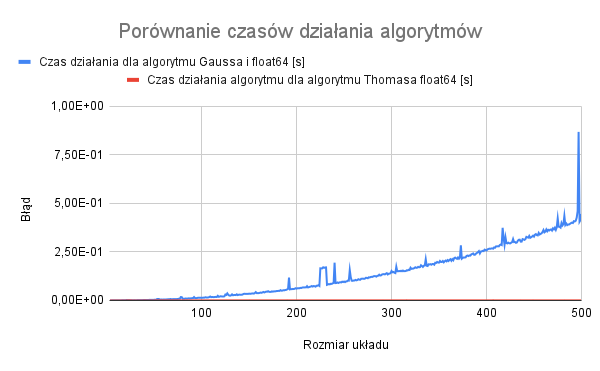
\includegraphics[width=\textwidth]{img14.png}
    \caption{Wykres czasów działania w zależności od przyjętej precyzji}
  \end{minipage}
  \hfill
  \begin{minipage}[b]{0.49\textwidth}
    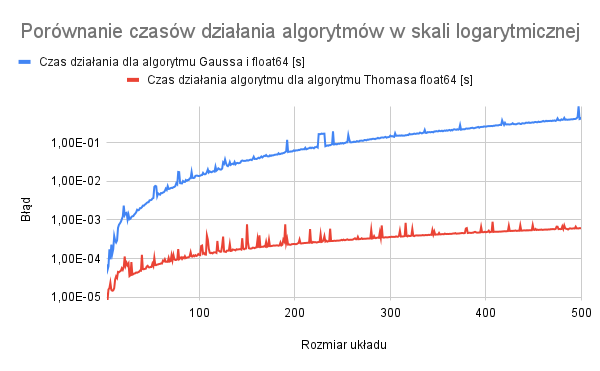
\includegraphics[width=\textwidth]{img15.png}
    \caption{Wykres czasów działania w skali logarytmicznej w zależności od przyjętej precyzji}
  \end{minipage}
\end{figure}

Zmiana precyzji nie wpłynęła na współczynnik uwarunkowania układu, który ponownie wynosi:

\[k(A) = 1.16\]

\newpage

\section{Wnioski}

\begin{enumerate}
    \item Na podstawie przeprowadzonych testów można zauważyć, że uwarunkowanie układu ma duży wpływa na dokładnośc otrzymanego przybliżenia.
    \item W niektórych przypadkach wyniki dla 64 bitowej precyzji są "o niebo" \ lepsze od wyników dla 32 bitowej precyzji
    \item Algorytm Thomasa jest znacznie szybszy od algorytmu Gaussa, jednek ten drugi jest bardziej uniwersalny.
\end{enumerate}

\section{Źródła}

\begin{enumerate}
    \item Wykład z przedmiotu MOwNiT prowadzony przez Panią dr. Katarzynę Rycerz
    \item https://eduinf.waw.pl/inf/alg/001\_search/0076.php
    \item https://en.wikipedia.org/wiki/Tridiagonal\_matrix\_algorithm
\end{enumerate}

\end{document}


